\documentclass[a4paper,8pt,fleqn]{article}

%pacchetti
\newcommand*\Eval[3]{\left.#1\right\rvert_{#2}^{#3}}
\usepackage[T1]{fontenc}
\usepackage{titling}
\usepackage{titlesec}
\usepackage[utf8]{inputenc}
\usepackage{empheq}
%\usepackage{fontawesome}
\usepackage{physics}
\usepackage[usenames, dvipsnames]{color}
\usepackage{pgfplots,filecontents,amsmath}
\pgfplotsset{compat=1.5}
\usepackage{xcolor,colortbl}
\usepackage{listings,tabu}
\usepackage{tikz}
\usepackage{float}
\usepackage{mdframed}
\usepackage{pbox}
\usepackage{sectsty}
\definecolor{mygreen}{RGB}{28,172,0} 
\definecolor{mylilas}{RGB}{170,55,241}
\lstset{language=Matlab,%
    %basicstyle=\color{red},
    breaklines=true,%
    morekeywords={matlab2tikz},
    keywordstyle=\color{blue},%
    morekeywords=[2]{1}, keywordstyle=[2]{\color{black}},
    identifierstyle=\color{black},%
    stringstyle=\color{mylilas},
    commentstyle=\color{mygreen},%
    showstringspaces=false,%without this there will be a symbol in the places where there is a space
    numbers=left,%
    numberstyle={\tiny \color{black}},% size of the numbers
    numbersep=9pt, % this defines how far the numbers are from the text
    emph=[1]{for,end,break},emphstyle=[1]\color{red}, %some words to emphasise
    %emph=[2]{word1,word2}, emphstyle=[2]{style},    
}

\usepackage{chngcntr}
\usepackage{tcolorbox}
\usepackage{amssymb, amsfonts}
\usepackage{tabulary}
\usepackage{braket}
\usepackage{pgfplots}
\usepackage{multicol}
\usepackage{stackengine}
\pgfplotsset{width=10cm,compat=1.9}
\usetikzlibrary{arrows}
\usepackage{mathtools}
\usepackage{cancel}
\usepackage{array}
\usepackage{siunitx}
\usepackage{tabularx}
\usepackage{cases}
\usepackage[absolute]{textpos}
\usepackage[italian,english]{babel}

\usepackage[toc]{multitoc}
\renewcommand*{\multicolumntoc}{2}
\setlength{\columnseprule}{0.5pt}

\usepackage{blindtext}
\usepackage{graphicx}
\usepackage{soul}
\usepackage{eqnarray}
\usepackage{fancyhdr}
\pagestyle{fancy}
\usepackage{lastpage}
\usepackage{emptypage}
\usepackage{parcolumns}
\usepackage{color}
\usepackage{colortbl}
\usepackage{caption}
% \usepackage{enumerate}
\usepackage{ushort}
\usepackage{dsfont}
\usepackage{mathrsfs}
\usepackage{graphics}
\usepackage{epstopdf}
\usepackage{hyperref}
\usepackage{geometry}
\usepackage{multirow}
\usepackage{varwidth}
\usepackage{booktabs}
\usepackage{enumitem}
\usepackage{algorithm}
\usepackage{algpseudocode}
\definecolor{orange-red}{rgb}{1.0, 0.27, 0.0}
 \geometry{
 a4paper,
 left=8mm,
 right=8mm,
 top=13mm,
 bottom=8mm
 }
\setlength{\columnseprule}{0.1pt}
\setlength{\columnsep}{0.05\textwidth} 
\pagestyle{fancy}
\fancyhf{}
\fancyheadoffset{0mm}
\rhead{}
\lhead{}
\chead{Page \thepage\ of \pageref{LastPage}}

\newcommand{\m}{ \underline } 
\newcommand{\mm}[1]{\underline{\underline{#1}}}
%comando personalizzato
\newcommand{\der}{\partial}
\newcommand{\1}{\frac}
\newcommand{\dt}{\cfrac{\mathrm{d}}{\mathrm{d}t}}
\newcommand{\dtm}{\cfrac{\mathrm{d}^-}{\mathrm{d}t}}
\newcommand{\dtp}{\cfrac{\mathrm{d}^+}{\mathrm{d}t}}
\newcommand{\cd}{\cdot}
\numberwithin{equation}{section}
\newtheorem{theorem}{Theorem}
\newcommand{\stabilo}[2][yellow]{\mathchoice%
  {\colorbox{#1}{$\displaystyle#2$}}%
  {\colorbox{#1}{$\textstyle#2$}}%
  {\colorbox{#1}{$\scriptstyle#2$}}%
  {\colorbox{#1}{$\scriptscriptstyle#2$}}}%

\newcommand{\subto}{\text{s.t.}}

\definecolor{term}{RGB}{0,0,255}
\newcommand{\term}[1]{\color{term} #1\color{black}}

%---------------------------------------------------

\author{}
\graphicspath{{images/}}
\begin{document}
\begin{hyphenrules}{nohyphenation}

\begin{footnotesize}
\subsectionfont{\color{blue}} 
\subsubsectionfont{\color{RoyalBlue}}

\title{Computational Control - FS 2024}
\author{Aschari Eric, Mastroddi Giacomo, Muttoni Marco}
\maketitle

\tableofcontents
\end{footnotesize}

\newpage
\begin{mdframed}[backgroundcolor=red!20, frametitlerulewidth=0pt, innertopmargin=-2mm, innerbottommargin=2mm, skipabove=0mm]

\section{Other Controllers}
\end{mdframed}

\subsection{PID}
\begin{minipage}{0.33\textwidth}
    \begin{tcolorbox}[colframe=green!50!black, colback=green!5!white, title=Pros, left=0.5mm, right=0.5mm]
    \begin{itemize}[leftmargin=*]
        \item Simple
        \item Known tuning methods
        \item Low computations
    \end{itemize}
    \end{tcolorbox}
\end{minipage}
\begin{minipage}{0.33\textwidth}
    \begin{tcolorbox}[colframe=red!50!black, colback=red!5!white, title=Cons, left=0.5mm, right=0.5mm]
    \begin{itemize}[leftmargin=*]
        \item Reactive response
        \item SISO (and some MIMO with cascaded)
        \item Nonlinear
    \end{itemize}
    \end{tcolorbox}
\end{minipage}
\begin{minipage}{0.33\textwidth}
    \begin{tcolorbox}[colframe=gray!50!black, colback=gray!5!white, title=Examples, left=0.5mm, right=0.5mm]
    \begin{itemize}[leftmargin=*]
        \item Reference tracking
        \item Position control drones
        \item Flow, temperature heating, chemical
    \end{itemize}
    \end{tcolorbox}
\end{minipage}

\subsection{Frequency Domain Design}
\begin{minipage}{0.33\textwidth}
\begin{tcolorbox}[colframe=green!50!black, colback=green!5!white, title=Pros, left=0.5mm, right=0.5mm]
\begin{itemize}[leftmargin=*]
\item Stability analysis (e.g., Nyquist, Bode plots)
\item Robustness to model uncertainties
\item Effective in handling disturbances
\end{itemize}
\end{tcolorbox}
\end{minipage}
\begin{minipage}{0.33\textwidth}
\begin{tcolorbox}[colframe=red!50!black, colback=red!5!white, title=Cons, left=0.5mm, right=0.5mm]
\begin{itemize}[leftmargin=*]
\item Complex design process
\item Limited applicability for nonlinear systems: requires linear models
\end{itemize}
\end{tcolorbox}
\end{minipage}
\begin{minipage}{0.33\textwidth}
\begin{tcolorbox}[colframe=gray!50!black, colback=gray!5!white, title=Examples, left=0.5mm, right=0.5mm]
\begin{itemize}[leftmargin=*]
\item Control of power systems (stability)
\item Vibration analysis in mechanical systems
\item Filter design in communication systems
\end{itemize}
\end{tcolorbox}
\end{minipage}
\newpage
\begin{mdframed}[backgroundcolor=red!20, frametitlerulewidth=0pt, innertopmargin=-2mm, innerbottommargin=2mm, skipabove=0mm]

\section{Linear Quadratic Regulator LQR}
\end{mdframed}
\begin{minipage}{0.33\textwidth}
    \begin{tcolorbox}[colframe=green!50!black, colback=green!5!white, title=Pros, left=0.5mm, right=0.5mm]
    \begin{itemize}[leftmargin=*]
        \item Optimal control law
        \item Guaranteed stability of the closed-loop system
        \item Online computationally less expensive 
        \item Ideal for linear systems
        \item Flexibility with tuning weights
    \end{itemize}
    \end{tcolorbox}
\end{minipage}
\begin{minipage}{0.33\textwidth}
    \begin{tcolorbox}[colframe=red!50!black, colback=red!5!white, title=Cons, left=0.5mm, right=0.5mm]
    \begin{itemize}[leftmargin=*]
        \item Linear system model 
        \item Model accuracy 
        \item Non-quadratic cost
        \item Constraints 
        \item Robustness is limited
        \item Large memory for finite horizon
    \end{itemize}
    \end{tcolorbox}
\end{minipage}
\begin{minipage}{0.33\textwidth}
    \begin{tcolorbox}[colframe=gray!50!black, colback=gray!5!white, title=Examples, left=0.5mm, right=0.5mm]
    \begin{itemize}[leftmargin=*]
        \item Aircraft autopilot
        \item Path tracking mobile robots
        \item Infinite horizon: persistent tracking in process automation, satellite trajectory
    \end{itemize}
    \end{tcolorbox}
\end{minipage}\\ \\
In general, optimization problems are typically intractable:\\
\begin{minipage}[t]{0.4\textwidth}
 \begin{itemize}
    \item size of $u$ is too large.
    \item require an accurate model of the system.   
 \end{itemize}
\end{minipage}
\begin{minipage}[t]{0.6\textwidth}
 \begin{itemize}
    \item non-convex (between two solutions you don't get another solution).
    \item open-loop nature make them useless in the presence of disturbances. 
 \end{itemize}
\end{minipage}

\subsubsection*{Finite Horizon}
$\Rightarrow$ returns in a sequence of time-varying gain matrices.\\
Tractable optimization problem: Linear dynamics and Quadratic cost.
\begin{itemize}
    \item \textbf{Markovian state} representation:
        $\left\{
        \begin{aligned}
            &\text{Next state is linearly dependent only on current state: }x_{t+1} = A x_t + B u_t. \\
            &\text{Quadratic cost is additive over time: } \sum_t x_t^\top Q x_t + u_t^\top R u_t. \\
            &\text{Initial condition $x_0$ is known.}
        \end{aligned}
        \right.$
    \item The problem is convex and decomposable $\rightarrow$ solvable via \textbf{backward induction} (\textcolor{blue}{\textbf{Bellman Optimality Principle}}: An optimal policy has the property that whatever the initial state and the initial decisions are, the remaining decisions must constitute an optimal policy with regard to the state resulting from the first decision.)
    \begin{align*}
    V_t(x) = \min_{u_t, \ldots, u_{T-1}} &\sum_{s=t}^{T-1} ( \underbrace{x_s^\top Q x_s + u_s^\top R u_s}_{\text{running cost}} ) + \underbrace{x_T^\top S x_T}_{\text{terminal cost}} \\
    \text{s.t.} \quad x_{s+1} &= A x_s + B u_s, \quad s = t, \ldots, T-1 \\
    x_t &= x
    \end{align*}
    where the optimal control sequence is given by 
    \begin{align*}
        u_t &= \underbrace{-(R + B^\top P_{t+1} B)^{-1} B^\top P_{t+1} A}_{\Gamma_t} x_t \\
        P_{t-1} &= Q + A^\top P_t A - A^\top P_t B (R + B^\top P_t B)^{-1} B^\top P_t A, \quad P_T = S
    \end{align*}
\end{itemize}

\textbf{Considerations}
\begin{itemize}
    \item $V_t(x)$ is the value function.
    \item $V_t(x) = x^\top P_t x$ is quadratic, i.e $P \succeq 0$ and symmetric.
    \item $V_0(x_0)$ is the (total) optimal cost.
    \item The result is a linear feedback control law, i.e accounts for disturbances. 
    \item \begin{minipage}[t]{0.45\textwidth}
            \textbf{Offline computation}
            \begin{itemize}
                \item $n \times n$ matrix multiplications ($A$)
                \item $m \times m$ matrix inversion ($R$)
                \item $T$ iterations (horizon)
            \end{itemize}
         \end{minipage}\hfill
         \begin{minipage}[t]{0.45\textwidth}
            \textbf{Online computation}
            \begin{itemize}
                \item Storage of $T$ $m \times n$ matrices ($\Gamma$)
                \item $m \times n$ matrix multiplications ($\Gamma_t x_t$)
            \end{itemize}
        \end{minipage}
\end{itemize}

\newpage

\subsubsection*{Infinite Horizon}
$\Rightarrow$ returns a constant gain matrix.\\
Extension of the LQR to an infinite horizon $T = \infty$ for LTI persistent tracking and regulation problems.
\begin{itemize}
    \item The iteration 
    \begin{equation*}
        P_{t-1} = Q + A^\top P_t A - A^\top P_t B (R + B^\top P_t B)^{-1} B^\top P_t A, \quad P_0 = 0
    \end{equation*}
    converges, as \( t \to \infty \), to a solution \( P_\infty \succ 0 \) of the Algebraic Riccati Equation (ARE):
    \begin{equation*}
        P = Q + A^\top P A - A^\top P B (R + B^\top P B)^{-1} B^\top P A.
    \end{equation*}
    where the optimal feedback control is given by
    \begin{equation*}
        u_t = \underbrace{-(R + B^\top P_{\infty} B)^{-1} B^\top P_{\infty} A}_{\Gamma_\infty} x_t
    \end{equation*}
\end{itemize}

\textbf{Considerations}
\begin{itemize}
    \item The sequence \( P_0, P_{-1}, P_{-2}, \ldots \) is non-decreasing due to Bellman Optimality Principle.
    \item The sequence \( P_0, P_{-1}, P_{-2}, \ldots \) is upper-bounded because it converges towards zero.
    \item $(A,B)$ stabilizable and $(Q^{\frac{1}{2}},A)$ detectable then ARE has a unique $P_{\infty} \succeq 0$ and $A+BK_\infty$ is asy. stable.
    \item In practice: unstable modes need to be weighted in the cost function. 
    \item \begin{minipage}[t]{0.45\textwidth}
            \textbf{Offline computation}
            \begin{itemize}
                \item $n \times n$ matrix multiplications ($A$)
                \item $m \times m$ matrix inversion ($R$)
                \item "$\infty$" iterations (horizon)
            \end{itemize}
         \end{minipage}\hfill
         \begin{minipage}[t]{0.45\textwidth}
            \textbf{Online computation}
            \begin{itemize}
                \item Storage of one $m \times n$ matrix (less memory required!)
                \item $m \times n$ matrix multiplications ($\Gamma_t x_t$)
            \end{itemize}
        \end{minipage}
\end{itemize}

\newpage
\begin{mdframed}[backgroundcolor=red!20, frametitlerulewidth=0pt, innertopmargin=-2mm, innerbottommargin=2mm, skipabove=0mm]

\section{Model Predictive Control MPC}
\end{mdframed}
\subsection{MPC and Tracking MPC}
\begin{minipage}{0.33\textwidth}
    \begin{tcolorbox}[colframe=green!50!black, colback=green!5!white, title=Pros, left=0.5mm, right=0.5mm]
    \begin{itemize}[leftmargin=*]
        \item Optimal control law
        \item Guaranteed stability 
        \item Constraints
        \item Disturbance rejection via receding horizon
        \item LTI: parametrized OCP in $x_0$
        \item Markovian systems
    \end{itemize}
    \end{tcolorbox}
\end{minipage}
\begin{minipage}{0.33\textwidth}
    \begin{tcolorbox}[colframe=red!50!black, colback=red!5!white, title=Cons, left=0.5mm, right=0.5mm]
    \begin{itemize}[leftmargin=*]
        \item Linear system model
        \item Model accuracy 
        \item Computationally expensive \& need to happen in one time step (online)
        \item Discrete state space
        \item Steady-state error
        \item Input disturbances, process noise, multiplicative noise
    \end{itemize}
    \end{tcolorbox}
\end{minipage}
\begin{minipage}{0.33\textwidth}
    \begin{tcolorbox}[colframe=gray!50!black, colback=gray!5!white, title=Examples, left=0.5mm, right=0.5mm]
    \begin{itemize}[leftmargin=*]
        \item Reference tracking
        \item Cruise control, autonomous driving
        \item Planning tasks
    \end{itemize}
    \end{tcolorbox}
\end{minipage}\\ \\
It is a static (memoryless), nonlinear (non-continuous), time-invariant feedback control law. \\
It is computed by solving an optimization control problem (OCP) parametrized by the initial state $x_0$ (time-invariant) and uses a receding horizon (same horizon length).
\begin{alignat*}{2}
    \min_{u, x} \quad & \sum_{k=0}^{K-1} g_k(x_k, u_k) + g_K(x_K) &&\\
    \text{subject to} \quad & x_{k+1} = f(x_k, u_k), &&k = 0, \ldots, K-1 \\
    & x_0 = x &&\\
    & x_k \in \mathcal{X}_k, &&k = 0, \ldots, K \\
    & u_k \in \mathcal{U}_k, &&k = 0, \ldots, K-1 \\
    & {\color{orange}x(T) = x_{\text{terminal}}} && 
\end{alignat*}

\subsubsection*{\textcolor{black}{Considerations}}
\begin{itemize}
    \item Does not manage to solve every optimization problem (for example when the optimal input turns out to be a the end of the horizon and there is no terminal constraint).
    \item \begin{minipage}[t]{0.45\textwidth}
            \textbf{Offline computation of $u^\star_0(.)$}
            \begin{itemize}
                \item Extremely complex
                \item Abundant computation power
                \item Large memory requirement (store all trajectories)
                \item Example: unconstrained linear MPC: first element of finite-time LQR
            \end{itemize}
         \end{minipage}\hfill
         \begin{minipage}[t]{0.45\textwidth}
            \textbf{Online computation of $u^\star_0(.)$}
            \begin{itemize}
                \item Tractable
                \item Limited time 
            \end{itemize}
        \end{minipage}
    \item Tracking is achieved by a change of coordinates $\left\{
        \begin{aligned}
            &\tilde{x} = x - x_\mathrm{ss} \\
            &\tilde{u} = u - u_\mathrm{ss}
        \end{aligned}
        \right.$
        \begin{itemize}
            \item Change of variables is inconsequential for LTI systems.
            \item $x_\mathrm{ss}$ is derived by first principles or from offline \textbf{steady state optimization} computation.
        \end{itemize}
\end{itemize}

\subsubsection*{Finite Horizon}
Discrete time system $x(k + 1) = A x(k) + B u(k)$ equilibrium point are defined by fixed points $x^\star = A x^\star + B u^\star$.\\ \\
\textcolor{blue}{Lyapunov Stability for Discrete-Time}\\
Let $x^\star = 0$ and $V$ be a continuous function such that
\begin{itemize}
    \item $V(0) = 0 \text{ and } V(x) > 0, \; \forall x \neq 0$
    \item $\Delta V(x(k)) \triangleq V(f(x(k))) - V(x(k)) < 0, \; \forall x(k) \in \mathcal{D}$
    \item $V$ radially unbounded: $\|x\| \to \infty \Rightarrow V(x) \to \infty$
\end{itemize}
$\Rightarrow$ then the origin is $\textbf{globally asy. stable}$.

\subsubsection*{\textcolor{orange}{Terminal constraint}\textcolor{black}{: $x(T) = x_{\text{terminal}}$}}
\begin{minipage}{0.58\textwidth}
    \begin{align*}
        W(x_{k+1}) &= \min \sum_{s=k+1}^{k+K} g(x_\mathrm{ss}, u_\mathrm{ss}) \\
        &= \min \sum_{s=k}^{k+K-1} g(x_\mathrm{ss}, u_\mathrm{ss}) - g(x_k, u_k) + \cancel{g(x_{k+K}, u_{k+K})})\\
        W(x_{k+1}) &\leq W(x_k) - g(\tilde{x}_k, \tilde{u}_k) \leq W(x_k)
    \end{align*}

    \subsubsection*{\textcolor{black}{Considerations}}
    \begin{itemize}
        \item Stability can be lost when receding horizon is too short or when full state is not available.
        \item Other sufficient conditions to guarantee MPC stability
            \begin{itemize}
                \item Terminal cost function: $\phi(x(T))$
                \item Terminal constraint set: $x(T) \in \mathcal{X}_\text{terminal}$
                \item Large receding horizon $K$
            \end{itemize}
    \end{itemize}
\end{minipage}
\begin{minipage}{0.38\textwidth}
    \begin{figure}[H]
        \centering
        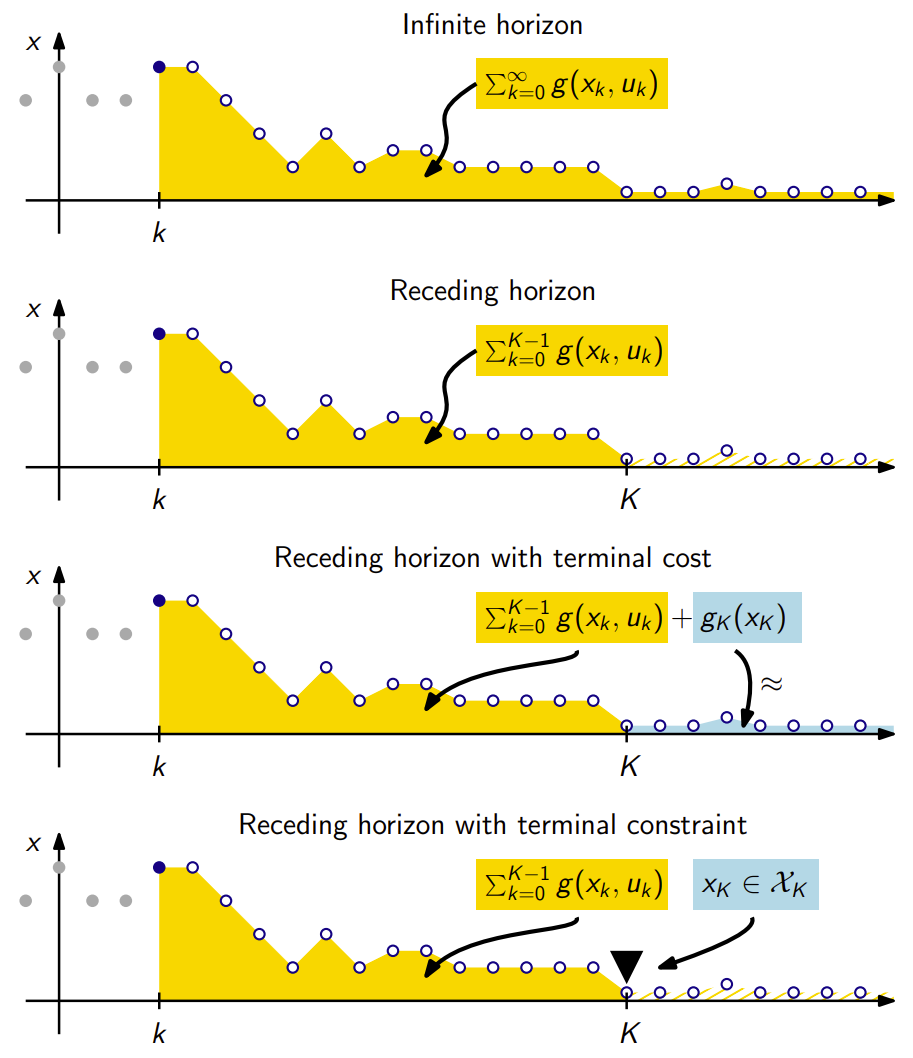
\includegraphics[width=0.9\columnwidth]{images/mpc.png}
    \end{figure}
\end{minipage}

\hrule

\subsubsection{Incremental MPC}
\begin{figure}[H]
    \centering
    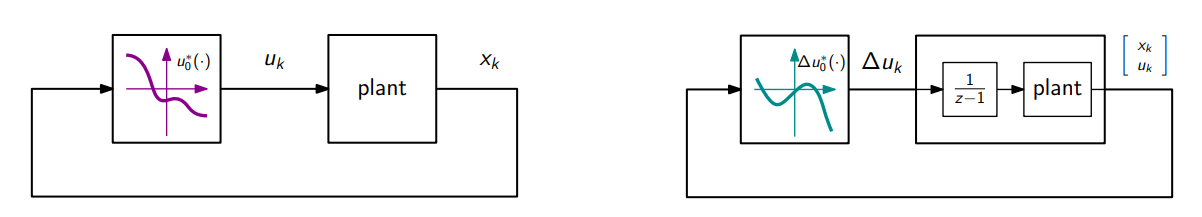
\includegraphics[width=0.8\linewidth]{images/incrementalMPC.png}
\end{figure}
\begin{minipage}[t]{0.48\textwidth}
    \textbf{Problems}:
    \begin{itemize}
        \item MPC will \textbf{not} achieve $x_\mathrm{ss}=0$ if a non-zero steady-state input is needed, because it inherently minimizes the input effort.
        \item Fragile against input disturbances, process noise, multiplicative noise.
        \item Low input can cause numerical issues.
    \end{itemize}
\end{minipage}
\begin{minipage}[t]{0.48\textwidth}
    \textbf{Solutions}:
    \begin{itemize}
        \item \textbf{Robustness}: Augment the plant with input integrator $\frac{1}{z-1}$ (if not present): more robust against disturbances and noise.
        \item \textbf{Numerical stability}: By penalizing $\Delta u_k = u_{k+1} - u_k$.
    \end{itemize}
\end{minipage}


\newpage

\subsection{Robust MPC}
\begin{minipage}{0.33\textwidth}
    \begin{tcolorbox}[colframe=green!50!black, colback=green!5!white, title=Pros, left=0.5mm, right=0.5mm]
    \begin{itemize}[leftmargin=*]
        \item Noise rejection ensuring feasible constraints
        \item Uncertainties within model
    \end{itemize}
    \end{tcolorbox}
\end{minipage}
\begin{minipage}{0.33\textwidth}
    \begin{tcolorbox}[colframe=red!50!black, colback=red!5!white, title=Cons, left=0.5mm, right=0.5mm]
    \begin{itemize}[leftmargin=*]
        \item Info about the noise/disturbance
        \item Open-loop: too conservative
        \item Closed-loop: difficult to find a parametrization
    \end{itemize}
    \end{tcolorbox}
\end{minipage}
\begin{minipage}{0.33\textwidth}
    \begin{tcolorbox}[colframe=gray!50!black, colback=gray!5!white, title=Examples, left=0.5mm, right=0.5mm]
    \begin{itemize}[leftmargin=*]
        \item Feasibility \& robustness: aerospace
        \item Reliability \& safety: driver assistant
        \item Power grids
    \end{itemize}
    \end{tcolorbox}
\end{minipage}\\ \\
\textbf{Problems:}
\begin{itemize}
    \item Cannot achieve zero tracking error due to the lack of an integrator.
    \item Neglected exogenous disturbances: \qquad $x_{k+1} = f(x_k, u_k, w_k)$
    \item Model mismatch: \qquad $x_{k+1} = \tilde{f}(x_k, u_k)$
    \item Missing dynamics / non-Markovianity: \qquad $
    \begin{cases}
        x_{k+1} = f(x_k, z_k, u_k) \\
        \textcolor{red}{z_{k+1} = f_z(x_k, z_k, u_k)}
    \end{cases}
    $
    \item Linearization: \qquad $x_{k+1} = \tilde{A}x_k + \tilde{B}u_k$
    \item And more: time discretization, quantization, time-varying parameters
\end{itemize}

\subsubsection{Disturbance Rejection in MPC}
\begin{figure}[H]
    \centering
    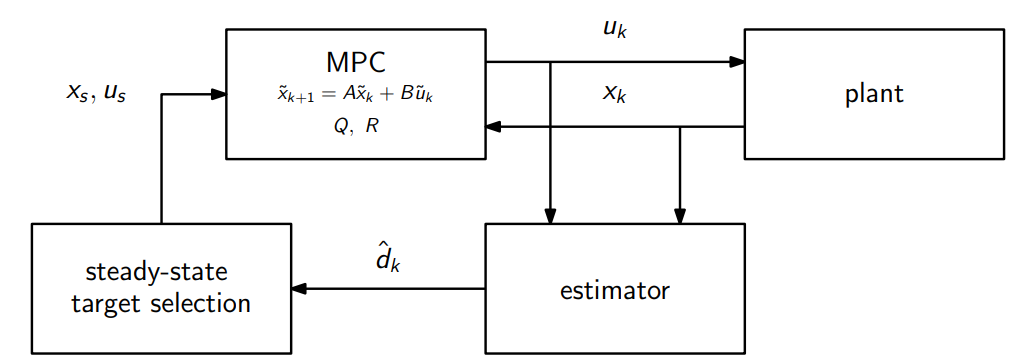
\includegraphics[width=0.6\linewidth]{images/distMPC.png}
\end{figure}
\textbf{Solutions:}
\begin{itemize}
    \item Model the disturbance as constant: \quad $\begin{bmatrix}
    x_{k+1} \\
    d_{k+1}
    \end{bmatrix}
    =
    \begin{bmatrix}
    A & B_d \\
    0 & I
    \end{bmatrix}
    \begin{bmatrix}
    x_k \\
    d_k
    \end{bmatrix}
    +
    \begin{bmatrix}
    B \\
    0
    \end{bmatrix}
    u_k$
    \item Predict of $x_{k+1}$ based on measurements $x_k, u_k$ and \textcolor{magenta}{estimate $\hat{d}_k$}: \quad $\hat{x}_{k+1} = A x_k + B u_k + \textcolor{magenta}{B_d \hat{d}_k}$
    \item Correct based on the prediction error: \quad $\hat{d}_{k+1} = \hat{d}_k + L \left( x_k - \hat{x}_k \right)$
    \item Select steady-state closer to specifications:
    \begin{align*}
    \min_{x_\mathrm{ss}, u_\mathrm{ss}} \quad & \| x_\mathrm{ss} - x_{\text{spec}} \|_{Q_\mathrm{ss}}^2 + \| u_\mathrm{ss} - u_{\text{spec}} \|_{R_\mathrm{ss}}^2 \\
    \text{subject to} \quad & \begin{bmatrix} I - A & -B \end{bmatrix} \begin{bmatrix} x_\mathrm{ss} \\ u_\mathrm{ss} \end{bmatrix} = \textcolor{magenta}{B_d \hat{d}_k} \\
    & x_\mathrm{ss} \in \mathcal{X} \\
    & u_\mathrm{ss} \in \mathcal{U}
    \end{align*}
\end{itemize}

\hrule

\subsubsection{Robust MPC}
\begin{minipage}[t]{0.48\textwidth}
\textbf{Closed-loop solution:}
\begin{itemize}
    \item Constructs a \textbf{feedback control} $u_1(x_1), \ldots, u_K^\star(x_K)$
    \item \textcolor{red}{Computationally intractable} (except for soft-constrained min-max LQR: worst-case scenario)
    \item \textcolor{ForestGreen}{Optimal}: all past information about the disturbance is used at each stage $k$
    \[
    \hat{w}_k = D^\dagger(x_{k+1} - A x_k - B u_k)
    \]
    \item \textbf{Dynamic programming} automatically returns the desired control law $u_0^\star(x)$ from offline computation.
    \item Corresponds to infinite-time optimal control at the limit $K \rightarrow \infty$.
\end{itemize}
\end{minipage}
\hfill
\begin{minipage}[t]{0.48\textwidth}
\textbf{Open-loop solution:}
\begin{itemize}
    \item Constructs an \textbf{input sequence} $u_0, u_1, \ldots, u_K$
    \item \textcolor{ForestGreen}{Computationally tractable} (convex optimization problem) but often \textbf{unfeasible}
    \item \textcolor{red}{Too conservative}: no past information about the disturbance is used except for the information available at $k=0$
    \item The desired control law $u_0^\star(x)$ is obtained by parametrizing the online optimization problem in $x$
\end{itemize}
\end{minipage}\\ \\

\hrule

\subsubsection{Feedback MPC}
A trade-off of the two solutions above: affine control law \quad $\boxed{u_k = v_k + Lx_k}$
\begin{itemize}
    \item $v_k$: Open-loop (feedforward) sequence/optimal policy
    \item $L$: Closed-loop (feedback) gain: rejects disturbances: \quad $x_{k+1} = (A+BL)x_k + Bv_k + Dw_k$
    \begin{itemize}
        \item $A+BL$ Hurwitz
        \item $L$ designed offline (can use Riccati by relaxing constraints of MPC)
    \end{itemize}
\end{itemize}
Alternative: optimize both $v$ and $L$ online $\rightarrow$ computationally complex $\rightarrow$ Tube MPC.

\newpage

\subsection{Economic MPC EMPC}
\begin{minipage}{0.33\textwidth}
    \begin{tcolorbox}[colframe=green!50!black, colback=green!5!white, title=Pros, left=0.5mm, right=0.5mm]
    \begin{itemize}[leftmargin=*]
        \item Considers complex metrics
        \item Efficient trajectories (transients)
        \item Linear program for linear $\ell$
        \item Future feasibility with steady-state terminal constraint
    \end{itemize}
    \end{tcolorbox}
\end{minipage}
\begin{minipage}{0.33\textwidth}
    \begin{tcolorbox}[colframe=red!50!black, colback=red!5!white, title=Cons, left=0.5mm, right=0.5mm]
    \begin{itemize}[leftmargin=*]
        \item More difficult to solve (not convex)
        \item Balancing economic objectives requires trade-offs
        \item Stability not guaranteed
    \end{itemize}
    \end{tcolorbox}
\end{minipage}
\begin{minipage}{0.33\textwidth}
    \begin{tcolorbox}[colframe=gray!50!black, colback=gray!5!white, title=Examples, left=0.5mm, right=0.5mm]
    \begin{itemize}[leftmargin=*]
        \item Efficiency tasks
        \item Processes: furnace, chemical industry
        \item Logistics, supply chain
    \end{itemize}
    \end{tcolorbox}
\end{minipage}\\ \\
It considers a \textbf{continuous} and \textbf{lower bounded} stage cost $\ell(x,u)$ (e.g. linear functions) that represents economic losses, energy use, cost of material, \ldots
\begin{align*}
    \min_{u, x} \quad & \sum_{k=0}^{K-1} \ell(x_k, u_k) \\
    \text{subject to} \quad & x_{k+1} = f(x_k, u_k), \quad k = 0, \ldots, K-1 \\
    & x_0 = x \\
    & x_k \in \mathcal{X}_k, \quad k = 0, \ldots, K \\
    & u_k \in \mathcal{U}_k, \quad k = 0, \ldots, K-1
\end{align*}
Alternative: \textbf{Steady-state optimization} problem and \textbf{tracking MPC} to follow reference:\\
\begin{minipage}[t]{0.48\textwidth}
    \textbf{\textcolor{LimeGreen}{Advantages}}
    \begin{itemize}
        \item Easier to use $\ell(x,u)$
    \end{itemize}
\end{minipage}
\begin{minipage}[t]{0.48\textwidth}
    \textbf{\textcolor{red}{Disadvantages}}
    \begin{itemize}
        \item Suboptimal solution.
        \item Cost is not reduced during system transients.
        \item Does not respond efficiently to disturbances. (Traffic example: offline compute $x_\mathrm{ss}, u_\mathrm{ss}$, but if there's an incident, they do not adapt to the new situation.)
    \end{itemize}
\end{minipage}\\
% \subsubsection*{\textcolor{black}{Considerations}}
% \begin{itemize}
%     \item Alternatively: \textbf{\textcolor{ForestGreen}{easier}} to use $\ell(x,u)$ to solve the \textbf{steady-state optimization} problem and \textbf{tracking MPC} to track, \textbf{\textcolor{red}{but}}
%         \begin{itemize}
%             \item Suboptimal solution.
%             \item Cost is not reduced during system transients.
%             \item Does not respond efficiently to disturbances. (Traffic example: offline compute $x_\mathrm{ss}, u_\mathrm{ss}$, but if there's an incident, they do not adapt to the new situation.)
%         \end{itemize}
% \end{itemize}
\subsubsection*{Infinite Horizon}
\begin{itemize}
    \item Economic interpretation (continuous processes, long-term gains, \ldots).
    \item May not drive the system to an equilibrium (not necessarily a problem).
    \item \textcolor{ForestGreen}{Boundedness} is guaranteed by the constraints (feasible future trajectory).
    \item \textcolor{red}{Computationally} intense due to infinite horizon. 
\end{itemize}
\subsubsection*{Finite Horizon}
\begin{itemize}
    \item \textcolor{ForestGreen}{Computationally} tractable.
    \item \textcolor{red}{Unstable trajectories} can emerge: cheap trajectory now, expensive fix later.
    \item \textcolor{red}{Infeasibility} at the end of the control horizon. 
\end{itemize}
\subsubsection*{\textcolor{orange}{Terminal constraint}\textcolor{black}{: $(x_\mathrm{ss}, u_\mathrm{ss})$}}
\begin{itemize}
    \item \textcolor{ForestGreen}{Computationally} more tractable.
    \item \textcolor{ForestGreen}{Future feasibility}.
    \item \textcolor{orange}{Stability} is \textbf{not guaranteed} as it was for MPC because $\ell(x,u)$ is not minimized at steady state. Nonetheless, asymptotic stability is \textbf{not desired} when using EMPC, such that it produces trajectories that are \textbf{efficient and economical}  (also limit cycles/periodic orbits) and do not converge to an equilibrium, which exhibits a higher cost.
    \item Even in the case in which the system converges to the steady state, EMPC produces \textbf{efficient}  trajectories to the equilibrium (theorem).
\end{itemize}
\textcolor{red}{\textbf{Note}}: stronger conditions are required to guarantee asy. stability.
\newpage
\begin{mdframed}[backgroundcolor=red!20, frametitlerulewidth=0pt, innertopmargin=-2mm, innerbottommargin=2mm, skipabove=0mm]

\section{System ID \& Data-enabled Predictive Control DeePC}
\end{mdframed}
\begin{minipage}{0.33\textwidth}
    \begin{tcolorbox}[colframe=green!50!black, colback=green!5!white, title=Pros, left=0.5mm, right=0.5mm]
    \begin{itemize}[leftmargin=*]
        \item Model-free
        \item More robust on noise
        \item No state estimator needed
        \item Many uses for predictor: filtering, control, recover missing data, prediction/simulation
    \end{itemize}
    \end{tcolorbox}
\end{minipage}
\begin{minipage}{0.33\textwidth}
    \begin{tcolorbox}[colframe=red!50!black, colback=red!5!white, title=Cons, left=0.5mm, right=0.5mm]
    \begin{itemize}[leftmargin=*]
        \item Computationally complex: $2n+K$ decision variables
        \item Larger memory footprint: data
        \item Based on LTI systems
        \item Mobel-based better if a state is known
        \item SysID incorporates available system info
        \item Hard and expensive to get data
    \end{itemize}
    \end{tcolorbox}
\end{minipage}
\begin{minipage}{0.33\textwidth}
    \begin{tcolorbox}[colframe=gray!50!black, colback=gray!5!white, title=Examples, left=0.5mm, right=0.5mm]
    \begin{itemize}[leftmargin=*]
        \item Temperature regulation
        \item Smart grid
        \item Medical devices
        \item Trading, price prediction and optimization
    \end{itemize}
    \end{tcolorbox}
\end{minipage}

\subsection{System Identification SysID}
Goal: find \textbf{minimal} (controllable \& observable) \textbf{realization} (state-space representation) given input-output data (not unique!).\\ \\
\begin{minipage}{0.43\textwidth}
    \begin{align*}
        x_k &= \underbrace{A^k x_0}_{\text{free response}} + \underbrace{\sum_{j=0}^{k-1} A^{k-1-j} B u_j + \sum_{i=0}^{k-1} A^{k-1-i} D_w w_i}_{\text{convolution}} \\
        y_k &= Cx_k + \underbrace{D u_k}_{\text{feedthrough}}
    \end{align*}
\end{minipage}
\begin{minipage}{0.53\textwidth}
    \begin{itemize}
    \item For a LTI, the impulse response is a complete representation of the input-output relation, as we can combine responses (superposition).
    \item \textcolor{blue}{\textbf{Markov Parameters}}: sequence of $\stabilo{CA^{k-1}B} \in \mathbb{R}^{p \times m} \quad k > 0$ where each element represent the output $i$ to an unit impulse on input $j$.
    \item At least $m$ impulse experiments are necessary to estimate them (needed to get matrix $B$).
    \end{itemize}
\end{minipage}

\subsubsection{Reachability - Controllability}
Investigate all states that can be reached at time $\tau$ starting at $x(0)=0$.
\begin{equation*}
    \stabilo{\mathcal{C}_n = [B \; AB \; A^2B \; A^3B \; \ldots \; A^{n-1}B ]} \quad \in \mathbb{R}^{n \times n} \qquad \text{Reachable: full row rank} \Leftrightarrow \text{rank}(\mathcal{C}_n)=n 
\end{equation*}
\begin{itemize}
    \item For linear-continuous time: set of reachable states = set of controllable states. \\
    System is completely reachable $\Rightarrow$ System completely controllable. 
    \item Differences between controllability and reachability: 
    \begin{itemize}
        \item \textbf{Compl. controllable}: may be kept to the origin, starting at any initial condition.
        \item  \textbf{Compl. reachable}: can only be brought to a certain point $x(T)$, but cannot be forced to stay there for $t>T$.
    \end{itemize}
\end{itemize}
\textbf{Considerations}
\begin{itemize}
    \item Scalar input creates column vector matrices $A, AB,\ldots \Rightarrow$ need $n$ steps for full rank
    \item Compl. controllable in less than $n$, if input $u$ is \textbf{not} scalar.
    \item Not compl. controllable in $n$ steps $\Rightarrow$ more steps won't help (linearly dep. on previous ones)
    \item Input sequence to reach target state $x_n = \mathcal{C}_n\begin{bmatrix}
    u_{n-1} \\
    \vdots \\
    u_0
    \end{bmatrix}$ if $\begin{cases} 
        \text{invertible} &\mathcal{C}_n^{-1} \\ 
        \text{non-invertible} &\mathcal{C}_n^T(\mathcal{C}_n\mathcal{C}_n^T)^{-1} \quad (\text{smallest norm})
        \end{cases}$ 
\end{itemize}

\subsubsection{Observability}
Reconstruct the initial condition $x(0)$ by analyzing only the output $y(t)$.
\begin{equation*}
    \stabilo{\mathcal{O}_n =
    \begin{bsmallmatrix}
    C \\ CA \\ CA^2 \\ \vdots \\ CA^{n-1}
    \end{bsmallmatrix}} \quad \in \mathbb{R}^{n \times n}
    \qquad \text{Observable: full column rank} \Leftrightarrow \text{rank}(\mathcal{O}_n) = n 
\end{equation*}
\textbf{Considerations}
\begin{itemize}
    \item Scalar input creates row vector matrices $C, CA,\ldots \Rightarrow$ need $n$ steps for full rank
    \item Compl. observable in less than $n$, if input $u$ is \textbf{not} scalar
    \item Not observable in $n$ steps $\Rightarrow$ more steps won't help (linearly dep. on previous ones)
    \item Initial state to produce target output sequence $\begin{bmatrix}
    y_0 \\
    \vdots \\
    y_{L-1}
    \end{bmatrix} = \mathcal{O}_L x_0$ if $\begin{cases} 
        L<n \text{ non-inv.} &\mathcal{O}_L^T(\mathcal{O}_L\mathcal{O}_L^T)^{-1} \quad (\text{smallest norm}) \\ 
        L=n \text{ invertible} &\mathcal{O}_n^{-1} \\ 
        L>n \text{ overdet.} & \text{not all } y \text{ are valid}
        
        \end{cases}$ 
\end{itemize}

\subsubsection{Hankel Matrix}
Hankel matrix composed of Markov parameters: $\stabilo{\mathcal{H} = \mathcal{O}\mathcal{C}}$ \\
\textbf{Ho-Kalman algorithm} (extended):
\begin{enumerate}
    \item Construct $\mathcal{H}_{k,l}$:
    \begin{itemize}
        \item Collect impulse responses as Markov parameters
    \item Estimate $k,l > n$: stop adding Markov parameters once rank $n$ is reached (rank $\mathcal{O}$ and $\mathcal{C}$ is $n$ such that they are compl. observable and controllable and automatically rank $\mathcal{H}$ is $n$)
    \end{itemize}
    \item Factorize $\mathcal{H}_{k,l}$ in $\mathcal{O}_k\mathcal{C}_l$:
    \begin{itemize}
        \item SVD: \quad $\mathcal{H}_{k,\ell} = 
        \begin{bmatrix}
        \color{red}{\mathbf{U}_1} & \mathbf{U}_2
        \end{bmatrix}
        \begin{bmatrix}
        \color{red}{\Sigma_1} & 0_{r \times n-r} \\
        0_{m-r \times r} & 0_{m-r \times n-r}
        \end{bmatrix}
        \begin{bmatrix}
        \color{blue}{\mathbf{V}_1} \\ \mathbf{V}_2
        \end{bmatrix}^{\top}
        = \mathbf{U}_1 \Sigma_1 \mathbf{V}_1^{\top}$ \qquad $U \in \mathbb{R}^{m\times m}$, $V \in \mathbb{R}^{n\times n}$
        \item $\mathcal{H}_{k,l} = \underbrace{\mathbf{U}_1 \Sigma_1^{1/2}}_{\textcolor{ForestGreen}{\mathcal{O}_k}} \underbrace{\Sigma_1^{1/2} \mathbf{V}_1^{\top}}_{\textcolor{orange}{\mathcal{C}_{l}}}$
        \item Shift $\mathcal{H}_{k,l}^\uparrow$ to get A
    \end{itemize}
    \item Derive $A,B,C$: \quad $A = \mathcal{O}_k^\dagger\mathcal{H}_{k,l}^\uparrow\mathcal{C}_l^\dagger$ \qquad $B$ from $\textcolor{orange}{\mathcal{C}_l}$ \qquad $C$ from $\textcolor{ForestGreen}{\mathcal{O}_k}$
\end{enumerate}

\hrule

\subsection{Behavioral Representation}
\begin{minipage}{0.68\textwidth}
    \[
        \begin{bmatrix}
        y_0 \\
        y_1 \\
        y_2 \\
        \vdots \\
        y_{L-1}
        \end{bmatrix}
        =
        \underbrace{
        \begin{bmatrix}
        C \\
        CA \\
        CA^2 \\
        \vdots \\
        CA^{L-1}
        \end{bmatrix}
        }_{\mathcal{O}_L \in \mathbb{R}^{Lp \times n}}
        x_0
        +
        \underbrace{
        \begin{bmatrix}
        0 & 0 & \cdots & 0 \\
        CB & 0 & \cdots & 0 \\
        CAB & CB & \cdots & 0 \\
        \vdots & \vdots & \ddots & \vdots \\
        CA^{L-2}B & CA^{L-3}B & \cdots & CB & 0
        \end{bmatrix}
        }_{\mathcal{G}_L \in \mathbb{R}^{Lp \times Lm}}
        \begin{bmatrix}
        u_0 \\
        u_1 \\
        u_2 \\
        \vdots \\
        u_{L-1}
        \end{bmatrix}
    \]
\end{minipage}
\begin{minipage}{0.28\textwidth}
    $\mathcal{O}_L$: extended observability matrix \\
    (free evolution of the system) \\
    $\mathcal{G}_L$: convolution matrix
    (forced evolution of the system)
\end{minipage}\\ \\
\textbullet \; $\textbf{y}_L - \mathcal{G}_L \textbf{u}_L = \mathcal{O}_L x_0$ \quad solved if $\textbf{y}_L - \mathcal{G}_L \textbf{u}_L$ is in the \textbf{column image} of $\mathcal{O}_L$: $\begin{cases} 
    Lm<n &\text{underdetermined} \\ 
    Lm=n &\text{ invertible}: x_0 = \mathcal{O}_n^{-1} (\textbf{y}_n - \mathcal{G}_n \textbf{u}_n) \\ 
    Lm>n &\text{ overdetermined}
\end{cases}$\\
\textbullet \; for $Lm > n$: $\mathbf{y}_L - \mathcal{G}_L \mathbf{u}_L$ \; needs to belong to a \textbf{subspace} spanned by $\mathcal{O}_L$ \\
    \textbullet \; All I/O trajectories ($\textbf{u}_L, \textbf{y}_L$) belong to 
    $\begin{array}{ll}
        \text{the \textbf{column image} of } \Lambda_L \\
        \text{a \textbf{subspace} of dimension } Lm + n 
    \end{array}$: \quad
    $\stabilo{\begin{bmatrix}
    \mathbf{u}_L \\
    \mathbf{y}_L
    \end{bmatrix}
    =
    \underbrace{
    \begin{bmatrix}
    I_{Lm} & \mathbf{0}_{Lm \times n} \\
    \mathcal{G}_L & \mathcal{O}_L
    \end{bmatrix}
    }_{\Lambda_L \in \mathbb{R}^{L(p+m) \times Lm+n}}
    \begin{bmatrix}
    \mathbf{u}_L \\
    x_0
    \end{bmatrix}} = \mathcal{H} \textbf{g}$ \\
\textbullet \; $\Lambda_L$ fully describes the system (I/O sequence compatible with the plant $= x_0$ such that $\ldots$)\\
$\rightarrow$ columns of $\Lambda_L$ are a basis of the subspace. \\
$\rightarrow$ columns of $\mathcal{H}$ are a basis of the subspace, with $\stabilo{\mathbf{g} \in \mathbb{R}^{Lm+n}}$ being a vector of coefficients.

\newpage

\subsubsection{Relations}
\begin{itemize}
    \item $\boxed{T_\mathrm{ini} = T_\mathrm{past}}$ length of the past data points used to initialize the problem $\begin{cases}
            \text{For SISO:} & T_\mathrm{ini} \geq n \\
            \text{For MIMO:} & T_\mathrm{ini} \geq \ell \ (\text{lag } \ell \leq n)
        \end{cases}$
    \item $\boxed{T_\mathrm{fut} = K}$ prediction horizon or the length of the future trajectory.
    \item $\boxed{L = T_\mathrm{ini} + T_\mathrm{fut}}$ 
    total length of the trajectory.
    \item $\boxed{T \geq (m + 1) \cdot (T_\mathrm{ini} + L) + n - 1}$ number of data points used to construct $\mathcal{H}$ $\begin{cases}
            \text{For SISO:} & T_\mathrm{min} = 2L + n - 1 \\
            \text{For MIMO:} & T_\mathrm{min} = (m+1) \cdot L + n - 1
        \end{cases}$
    \item $\boxed{\text{col}_\mathcal{H} \geq T - L + 1}$ number of columns
    \item $\boxed{\text{row}_\mathcal{H} = L \cdot (m + p)}$ number of rows
    \item $\boxed{\underset{\text{max}}{\operatorname{rank}}(\mathcal{H}) = Lm + n}$ rank maximum (SISO: $L+n = K+2n$)
\end{itemize}
\textbullet \; $Lm + n$ lin. ind. columns of $\mathcal{H}$ are chosen from data:

\begin{minipage}{0.43\textwidth}
    \[
    \mathcal{H}_{m \cdot L}(\textbf{u}_{\text{data}}) = 
    \begin{bmatrix}
    u_0 & u_1 & \cdots & u_{Lm+n-1} \\
    u_1 & u_2 & \cdots & u_{Lm+n-2} \\
    \vdots & \vdots & \ddots & \vdots \\
    u_{Lm-1} & u_{Lm} & \cdots & u_{2Lm+n-2}
    \end{bmatrix}
    \]
\end{minipage}
\begin{minipage}{0.43\textwidth}
    \[
    \mathcal{H}_{p \cdot L}(\textbf{y}_{\text{data}}) = 
    \begin{bmatrix}
    y_0 & y_1 & \cdots & y_{Lm+n-1} \\
    y_1 & y_2 & \cdots & y_{Lm+n-2} \\
    \vdots & \vdots & \ddots & \vdots \\
    y_{Lm-1} & y_{Lm}  & \cdots & y_{2Lm+n-2}
    \end{bmatrix}
    \]
\end{minipage}\\ \\
\textbf{Considerations}
\begin{itemize}
    \item \textbf{Persistence of excitation} in the collected data ensures full rank and that all dynamics are represented.
    \item Adding data to $\mathcal{H}$ ensures enough data in case $n$ is uncertain and all system modes have been exited.
    \item Ideally, $\mathcal{H}$ stops increasing after $mL+n$ (noiseless case).
\end{itemize}

\hrule

\subsection{DeePC}
\begin{minipage}{0.53\textwidth}
    \begin{align*}
        \underset{\textbf{u}, \textbf{y}, \textbf{g}, {\color{cyan}\boldsymbol{\sigma}}}{\operatorname{min}} \; & \sum_{k=0}^{K} \|\textbf{y}_k - \textbf{y}_\mathrm{ref} \|^2_Q + \|\textbf{u}_k - \textbf{u}_\mathrm{ref} \|_R^2 + {\color{red}\lambda_g \| \textbf{g} \|_1} + {\color{cyan}\lambda_\sigma \| \boldsymbol{\sigma} \|_1} \\
        \text{s.t.} \; & \underbrace{\begin{bmatrix}
        \mathcal{H}_{m \cdot L}(\textbf{u}_{\text{data}}) \\
        \mathcal{H}_{p \cdot L}(\textbf{y}_{\text{data}})
        \end{bmatrix}}_{\mathcal{H}} \textbf{g} = \begin{bmatrix}
        \textbf{u}_{\text{past}} \\
        \textbf{u}_{\text{fut}} \\
        \textbf{y}_{\text{past}} + {\color{cyan}\boldsymbol{\sigma}}\\
        \textbf{y}_{\text{fut}}
        \end{bmatrix} \\
        & \textbf{u}_k \in \mathcal{U}_k \quad \forall k \\
        & \textbf{y}_k \in \mathcal{Y}_k \quad \forall k \\
    \end{align*}
\end{minipage}
\begin{minipage}{0.43\textwidth}
    Against noise and/or nonlinearities: \\
    \textbullet \, \textcolor{red}{Regularized}/rank constraint: $\underset{\text{max}}{\operatorname{rank}}(\mathcal{H}) = Lm + n$: \\
    Prevent overfitting to noise/mismatches \\
    $\begin{cases} 
    \uparrow \lambda_g: &\text{fewer trajectories considered}\\ 
    \text{too high } \lambda_g: &\text{over-regulation}\\ 
    \downarrow \lambda_g: &\text{more trajectories considered} \\
    \text{too low } \lambda_g: &\text{irrelevant/incorrect info used}
    \end{cases}$ \\ \\
    \textbullet \, \textcolor{cyan}{Slack variable}: slightly relax constraint: \\ noise/mismatches in initial conditions \\
    $\begin{cases} 
    \uparrow \lambda_\sigma: &\text{more precise initial state selection}\\ 
    \text{too high } \lambda_\sigma: &\text{poor tracking: cost dominated by $\lambda_\sigma$}\\ 
    \downarrow \lambda_\sigma: &\text{more corrections possible} \\
    \text{too low } \lambda_\sigma: &\text{poor estimation, poor tracking}
    \end{cases}$ 
\end{minipage}
\newpage
\begin{mdframed}[backgroundcolor=red!20, frametitlerulewidth=0pt, innertopmargin=-2mm, innerbottommargin=2mm, skipabove=0mm]

\section{Markovian Decision Processes MDP - Optimal Control}
\end{mdframed}
\begin{minipage}{0.33\textwidth}
    \begin{tcolorbox}[colframe=green!50!black, colback=green!5!white, title=Pros, left=0.5mm, right=0.5mm]
    \begin{itemize}[leftmargin=*]
        \item Discretized state space
        \item Nonlinear dynamics
    \end{itemize}
    \end{tcolorbox}
\end{minipage}
\begin{minipage}{0.33\textwidth}
    \begin{tcolorbox}[colframe=red!50!black, colback=red!5!white, title=Cons, left=0.5mm, right=0.5mm]
    \begin{itemize}[leftmargin=*]
        \item Model-based in the form of transition probabilities
        \item Memory to store $\pi$ and $V$
    \end{itemize}
    \end{tcolorbox}
\end{minipage}
\begin{minipage}{0.33\textwidth}
    \begin{tcolorbox}[colframe=gray!50!black, colback=gray!5!white, title=Examples, left=0.5mm, right=0.5mm]
    \begin{itemize}[leftmargin=*]
        \item Traffic: number of vehicles per queue
        \item Stochastic processes: arrival of people, weather
        \item Fastest trajectory
        \item Games
    \end{itemize}
    \end{tcolorbox}
\end{minipage}
\begin{itemize}
    \item \textbf{\textcolor{cyan}{Model}} in form of probability transition: 
    $\begin{cases} 
        P: \mathcal{X} \times \mathcal{U} \times \mathcal{X} \rightarrow [0,1) \\ 
        {\color{cyan}P^u_{x,x'}} = \mathbb{P}[x'|x,u]
    \end{cases}$ \quad with set $\mathcal{X}$ of $N$ states and set $\mathcal{U}$ of $M$ inputs.
    \item \textbf{Markov property}: ${\color{cyan}P^u_{x,x'}}, \; \forall x'$ only depends on $x$ and $u$
    \item \textbf{Goal}: design a \textcolor{blue}{policy} to select $u \in \mathcal{U}$ on current $x \in \mathcal{X}$: 
    $\begin{cases} 
        \text{deterministic} &\mu: \mathcal{X} \rightarrow \mathcal{U} \\ 
        \text{stochastic } &\pi: \mathcal{X} \times \mathcal{U} \rightarrow [0,1) \quad \pi(x,u) = \mathbb{P}[u|x]
    \end{cases}$
    \item \textbf{\textcolor{orange}{Discounted} Bellman Equation (contractive)}: Dynamic programming to be solved via backward recursion:
    \begin{align*}
        V^{\textcolor{blue}{\pi}}_{k}(x) = {\color{orange}V^{\pi}(x)} &= \mathbb{E} \left[ \sum_{i=k}^{K = {\color{orange}\infty}} {\color{orange}\gamma^i} c_i \bigg| x_k = x \right] = \mathbb{E} \left[ c_k + \sum_{i=k+1}^{K = {\color{orange}\infty}} {\color{orange}\gamma^i} c_i \bigg| x_k = x \right] = \mathbb{E} \left[ c_k \big| x_k = x \right] + {\color{orange}\gamma} \mathbb{E} \left[ \sum_{i=k+1}^{K = {\color{orange}\infty}} c_i \bigg| x_k = x \right] \\
        &= \sum_{u} \textcolor{blue}{\pi_k(x, u)} \cdot \mathbb{E} \left[ c_k \big| x_k = x, u_k = u \right] + {\color{orange}\gamma} \sum_{u} \textcolor{blue}{\pi_k(x, u)} \cdot \mathbb{E} \left[ \sum_{i=k+1}^{K = {\color{orange}\infty}} c_i \bigg| x_k = x, u_k = u \right] \\
        &= \sum_{u} \textcolor{blue}{\pi_k(x, u)} \left[ \underbrace{\mathbb{E} \left[ c_k \big| x_k = x, u_k = u \right]}_{\color{teal}{C^u_x}} + {\color{orange}\gamma} \sum_{x'} {\color{cyan}P^u_{x,x'}} \underbrace{\mathbb{E} \left[ \sum_{i=k+1}^{K = {\color{orange}\infty}} c_i \bigg| x_{k+1} = x' \right]}_{V^{\textcolor{blue}{\pi}}_{k+1}(x') = {\color{orange}V^{\pi}(x')}} \right]
    \end{align*}
    $\rightarrow$ \textbf{Consistency equation}: Compute the \textcolor{red}{value function} $V$ of a \textcolor{blue}{policy} $\pi$ based on \textcolor{cyan}{model} $P^u_{x,x'}$ and (immediate observable) \textcolor{teal}{cost} $C_x^u$ (with an estimate of future cost $V^{\pi}(x')$). \\
    \textcolor{orange}{Infinite time}: Stationary (\textcolor{orange}{no $k$} for $V, \pi$), time invariant $C^u_x$ and $\pi$. \\
    \phantom{\textcolor{orange}{Infinite time}:} With discount factor $\gamma \in [0,1)$ to ensure finite cost (Bernoulli termination probability).
    \item \textbf{Bellman Optimality Principle/Equation}: optimal sequential decision problems \\
    \begin{minipage}[t]{0.48\textwidth}
        Optimal value/cost:
        \begin{align*}
            \textcolor{red}{V^\star_k(x)} &= \min_{\textcolor{blue}{\pi_k}} V^{\textcolor{blue}{\pi}}_{k}(x) \\
            &= \min_{\textcolor{blue}{\pi_k}} \sum_{u} \textcolor{blue}{\pi_k(x, u)} \left[ {\color{teal}C^u_x} + \sum_{x'} {\color{cyan}P^u_{x,x'}} V^{\textcolor{blue}{\pi}}_{k+1}(x') \right]
        \end{align*}
    \end{minipage}
    \begin{minipage}[t]{0.48\textwidth}
        Inductively:
        \[
        \textcolor{red}{V^\star_k(x)} = \min_{\textcolor{blue}{\pi_k}} \sum_{u} \textcolor{blue}{\pi_k(x, u)} \left[ {\color{teal}C^u_x} + \sum_{x'} {\color{cyan}P^u_{x,x'}} \textcolor{red}{V^\star_{k+1}(x')} \right]
        \]
    \end{minipage}\\ \\
    $\rightarrow$ Linear Program (LP) per $x$ with base case $V_K$. At each step, a $\pi$ is found.\\
    $\rightarrow$ Finite number of states and actions allows to tackle nonlinear stochastic systems with LP.
    \item For a \textbf{fixed policy} $\pi$, the MDP reduces to a \textcolor{blue}{\textbf{Markov Chain}} with transition probabilities $P^{\pi}_{x,x'}$ and stationary distribution $\bar{d}(x)$:
    \begin{equation*}
        P^{\pi} = \sum_u \mathbb{P}[x' | x, u]\pi(x, u) = \sum_u \pi(x, u) P^{u}_{x,x'}
    \end{equation*}
    Stationary point:
    \begin{equation*}
        d_{k+1}^{\top} = d_k^{\top} P^{\pi} \quad \implies \quad \boxed{\bar{d}^{\top} = \bar{d}^{\top} P^{\pi}}
    \end{equation*}
\end{itemize}

\begin{tcolorbox}[colframe=cyan!50!black, colback=cyan!5!white, title=Policy Iteration]
\textbf{\textcolor{blue}{Policy Evaluation}}: expensive: $\mathcal{O}(N^3+N^2M)$: inverse $+$ multiply $N \times N$ with $N \times 1$, $M$ times.
\begin{itemize}
    \item \textcolor{orange}{Infinite time}, \textbf{finite} MDP with $N$ states $\Rightarrow$ system of $N$ linear equations: \quad $\boxed{V^{\pi} = C^{\pi} + \gamma P^{\pi} V^{\pi}}$ \\
    with
    $\begin{cases}
        C^{\pi}(x) = \sum_{u} \textcolor{blue}{\pi(x, u)} {\color{teal}C^u_x} & \text{expected cost } N \times 1\\
        P^{\pi} = \sum_{u} \textcolor{blue}{\pi(x, u)} {\color{cyan}P^u_{x,x'}} & \text{expected transition probabilities (row-stochastic) } N \times N
    \end{cases}$ \\
    $\stabilo{V^{\pi} = (I - \gamma P^{\pi})^{-1} C^{\pi}}$ \qquad Always invertible (Perron-Frobenious see ATIC) and unique solution.
\end{itemize}

\textbf{\textcolor{LimeGreen}{Greedy Policy Improvement}}: easy: min over $M$ alternatives, $N$ times.
\begin{itemize}
    \item Always improve value ($V^{\pi'}(x) < V^{\pi}(x)$ unless $V^{\pi} = V^\star$) by deviating from current $\pi$ for one step $\textcolor{purple}{\nu}$ and then fall back to $\pi$:
    \[
    {\color{blue}\pi'(x, u)} = \arg \min_{\textcolor{purple}{\nu}} \sum_{u} \textcolor{purple}{\nu(x, u)} \left[ {\color{teal}C^u_x} + {\color{orange}\gamma} \sum_{x'} {\color{cyan}P^u_{x,x'}} V^{\color{blue}\pi}(x') \right]
    \]
\end{itemize}
\textbf{Convergence in finite number of steps} because the number of actions and states is finite.
\end{tcolorbox}

\begin{algorithm}[H]
\caption{Policy Iteration Algorithm}
\begin{algorithmic}[1]
    \State \textbf{Initialize} at a policy guess $\pi \gets \pi_0$
    \For{each iteration}
    \State $V \gets (I - \gamma P^{\pi})^{-1} C^{\pi}$ \Comment{Compute the value $V$ associated to the policy $\pi$}
    \State $\pi(x, u) \gets \arg \min_{\nu} \sum_{u} \nu(x, u) \left[ C^u_x + \gamma \sum_{x'} P^u_{x,x'} V(x') \right]$ \Comment{Greedy update of the policy to update $\pi$}
    \EndFor
\end{algorithmic}
\end{algorithm}

\begin{tcolorbox}[colframe=purple!50!black, colback=purple!5!white, title=Value Iteration]
Fixed point of the Bellman Optimality Equation: cheap: $\mathcal{O}(N^2M)$
\[
\textcolor{orange}{V^\star(x)} = \min_{\textcolor{blue}{\pi}} \sum_{u} \textcolor{blue}{\pi(x, u)} \left[ {\color{teal}C^u_x} + {\color{orange}\gamma} \sum_{x'} {\color{cyan}P^u_{x,x'}} \textcolor{orange}{V^\star(x')} \right]
\]
\textbf{Convergence asymptotically} (after $\infty$ iterations) with rate $\gamma$ to $V^\star$ (\textbf{contractive}).
\end{tcolorbox}

\begin{algorithm}[H]
\caption{Value Iteration Algorithm}
\begin{algorithmic}[1]
    \State \textbf{Initialize} at a value guess $V \gets V_0$
    \For{each iteration}
    \State $V(x) \gets \min_{\pi} \sum_{u} \pi(x, u) \left[ C^u_x + \gamma \sum_{x'} P^u_{x,x'} V(x') \right]$ \Comment{Apply the Bellman iteration}
    \EndFor
    \If{convergence}
    \State $\pi(x, u) \gets \arg \min_{\nu} \sum_{u} \nu(x, u) \left[ C^u_x + \gamma \sum_{x'} P^u_{x,x'} V(x') \right]$ \Comment{Extract the optimal policy $\pi^\star$ (greedy policy)}
    \EndIf
\end{algorithmic}
\end{algorithm}

\newpage

\begin{mdframed}[backgroundcolor=red!20, frametitlerulewidth=0pt, innertopmargin=-2mm, innerbottommargin=2mm, skipabove=0mm]
\section{Monte Carlo (Episodic) Learning}
\end{mdframed}
\begin{minipage}{0.33\textwidth}
    \begin{tcolorbox}[colframe=green!50!black, colback=green!5!white, title=Pros, left=0.5mm, right=0.5mm]
    \begin{itemize}[leftmargin=*]
        \item Model-free (based on collected data) \\
        $\rightarrow$ use simulator (cheap) or controlled environment
        \item Parametrization via neural networks
    \end{itemize}
    \end{tcolorbox}
\end{minipage}
\begin{minipage}{0.33\textwidth}
    \begin{tcolorbox}[colframe=red!50!black, colback=red!5!white, title=Cons, left=0.5mm, right=0.5mm]
    \begin{itemize}[leftmargin=*]
        \item Averaging state-action pairs of full episode renders learning slow/inefficient (chess: 1 bad move and all perfect)
        \item No param.: exp. increasing matrix
        \item Param. reduces DoF \& not solve Bellman equation
    \end{itemize}
    \end{tcolorbox}
\end{minipage}
\begin{minipage}{0.33\textwidth}
    \begin{tcolorbox}[colframe=gray!50!black, colback=gray!5!white, title=Examples, left=0.5mm, right=0.5mm]
    \begin{itemize}[leftmargin=*]
        \item Finance, managing portfolio
        \item Logistic inventory
        \item Drug development/simulation
    \end{itemize}
    \end{tcolorbox}
\end{minipage}\\ \\
\textcolor{red}{Quality function} $Q$ returns the expect future cost of taking action $u$ at state $x$ and apply policy $\pi$ afterwards.
\begin{itemize}
    \item \textbf{\textcolor{orange}{Discounted} Bellman Equation}:
    \begin{alignat*}{2}
        {\color{orange}V^{\pi}(x)} &= \sum_{u} \textcolor{blue}{\pi(x, u)} \underbrace{\left[ {\color{teal}R^u_x} + {\color{orange}\gamma} \sum_{x'} {\color{cyan}P^u_{x,x'}} {\color{orange}V^{\pi}(x')} \right]}_{{\color{orange}Q^{\pi}(x,u)}} \qquad && N \text{ states}\\
        {\color{orange}Q^{\pi}(x,u)} &= {\color{teal}R^u_x} + {\color{orange}\gamma} \sum_{x'} {\color{cyan}P^u_{x,x'}} \underbrace{\sum_{u'} \textcolor{blue}{\pi(x', u')} {\color{orange}Q^{\pi}(x', u')}}_{\color{orange}V^{\pi}(x')} = \mathcal{B}(Q) \qquad && N \text{ states} \times M \text{ actions}
    \end{alignat*}
    \item \textbf{Bellman Optimality Principle/Equation}:
    \begin{alignat*}{2}
        \textcolor{red}{V^\star(x)} &= \min_{\textcolor{blue}{u}} \left[ {\color{teal}R^u_x} + \sum_{x'} {\color{cyan}P^u_{x,x'}} \textcolor{red}{V^\star(x')} \right] = \min_u Q(x,u) \qquad &&
        \begin{aligned}
            &\textbf{Deterministic policy } \& \textcolor{orange}{\text{ infinite time}} \\
            &\rightarrow N \text{ nonlinear equations (min on finite set)}
        \end{aligned} \\
        \textcolor{red}{Q^\star(x,u)} &= {\color{teal}R^u_x} + \sum_{x'} {\color{cyan}P^u_{x,x'}} \left( \min_{\textcolor{blue}{u'}} \textcolor{red}{Q^\star(x', u')} \right) \qquad &&
        \begin{aligned}
            &\text{Swapped min with $\mathbb{E}$ (easier).}\\ 
            &\text{Both define implicitly optimal strategy.} 
        \end{aligned}
    \end{alignat*}
\end{itemize}

\begin{tcolorbox}[colframe=cyan!50!black, colback=cyan!5!white, title=Policy Iteration]
\textbf{\textcolor{blue}{Experimental Policy Evaluation}}: \textbf{No model}, from experiment/simulations (difficult and time consuming)
\begin{enumerate}
    \item Collect a (long) episode: \qquad $(x_0, u_0, r_0), \ (x_1, u_1, r_1), \ \ldots \ (x_T, u_T, r_T)$
    \item Compute the \textbf{empirical cost} \quad $g_0, g_1, \ldots, g_T$
    \item Interpret $g_k$ as a realization of the return in the \textbf{state-action pair} $x_k, u_k$
    \begin{align*}
        Q^{\pi}(x_k, u_k) &\approx g_k = \sum_{i=k}^{T} \gamma^{i-k} r_i \\
        Q^{\pi}(x, u) &= \frac{\sum_{t=1}^{T} 1[x_t = x, u_t = u] \, g_t}{\sum_{t=1}^{T} 1[x_t = x, u_t = u]} \qquad \text{in case of multiple visits}
    \end{align*}
    Ergodicity assumption: all states visited.
\end{enumerate}
\textcolor{red}{Note}: Policy evaluated ($Q$ computed) only at the end of the episode, when agent sees final outcome. \\
\textcolor{red}{Note}: The estimation does not satisfy Bellman equation (unless with $\infty$ data). \\
\textcolor{red}{Note}: Markovianity of the physical system not exploited to make computation of $Q$ more efficient $\rightarrow$ missing consistency.\\

\textbf{\textcolor{LimeGreen}{Greedy Policy Improvement}}: \textbf{No model} information needed:
\[
\stabilo{{\color{blue}\pi'(x, u)} = \arg \min_{\textcolor{purple}{\nu}} \sum_{u} \textcolor{purple}{\nu(x, u)} Q(x,u)}
\]
\textcolor{red}{Note}: Can find suboptimal solution: not learnt enough or optimal found and not exploring anymore.\\ \\
\textbf{Exploration and Exploitation}:\\
\begin{minipage}[t]{0.58\textwidth}
    \textcolor{LimeGreen}{$\epsilon$-greedy Policy Improvement}
    \[
    \pi(x, u) \gets
    \begin{cases}
    \arg \underset{u}{\min} Q(x, u) & \text{with probability } 1 - \epsilon \\
    \text{Uniform}(\mathcal{U}) & \text{with probability } \epsilon
    \end{cases}
    \]
    Large $\epsilon$ $\rightarrow$ more exploration
\end{minipage}
\begin{minipage}[t]{0.38\textwidth}
    \textcolor{LimeGreen}{Boltzmann Policy Improvement}
    \[
    \pi(x, u) \gets \frac{e^{-\beta Q(x, u)}}{\sum_{u} e^{-\beta Q(x, u)}}
    \]
    Small $\beta$ $\rightarrow$ more exploration
\end{minipage}
\begin{itemize}
    \item As learning progresses from episode to episode, $\epsilon \rightarrow 0$ or $\beta \rightarrow \infty$ (explore less, exploit more).
    \item If done “properly”, then with probability 1
    \begin{itemize}
        \item each state-action pair is visited \textbf{infinitely often}
        \item the policy converges to a \textbf{greedy policy}
    \end{itemize}
\end{itemize}
\end{tcolorbox}

\newpage
\subsection{Parametrization of $Q$}
\begin{itemize}
    \item In theory: memorize $Q$ in table $\rightarrow$ computationally infeasible (many state-action), intractable (continuous state-action).
    \item In practice: $\boxed{Q_\theta(x,u) = \phi^\top\theta = \Phi\theta}$ 
    $\begin{cases}
        \Phi \in \mathbb{R}^{NM \times d} & \text{basis functions} \\
        \theta \in \mathbb{R}^d &
    \end{cases}$
\end{itemize}
\begin{minipage}[t]{0.48\textwidth}
    \textbf{\textcolor{LimeGreen}{Advantages}}
    \begin{itemize}
        \item Smaller memory ($d$ instead of $NM$)
        \item Problem size is (apparently) independent from $N \rightarrow$ continuous state space
        \item A smart parametrization may allow to "guess" the Q function in state-action pairs that have not been observed (interpolation/extrapolation)
        \item Prior information on the problem may suggest a smart parametrization
    \end{itemize}
\end{minipage}
\begin{minipage}[t]{0.48\textwidth}
    \textbf{\textcolor{red}{Disadvantages}}
    \begin{itemize}
        \item Reduced degrees of freedom
        \item The solution to the Bellman equation for a given policy $\pi$ may not belong to $\mathcal{Q} = \{ Q^\theta, \theta \in \mathbb{R}^d \}$ (fixed point) because the solution is not of the same form.
        \item Possible consequences on
        \begin{itemize}
            \item convergence of policy iterations
            \item optimality of the limit
        \end{itemize}
        \item Computing $\theta$ that best approximates the data collected from an episode may be computationally expensive
    \end{itemize}
\end{minipage}\\
\begin{itemize}
    \item \textbf{Q-Bellman Equation} $\mathcal{B}(Q)$:
    \[
    \mathcal{B}(Q) = {\color{teal}R^u_x} + {\color{orange}\gamma} \underbrace{\sum_{x'} {\color{cyan}P^u_{x,x'}} \sum_{u'} \textcolor{blue}{\pi(x', u')}}_{T^{\pi}} {\color{orange}Q^{\pi}(x', u')} = R + \gamma T^\pi Q \quad \begin{cases}
        Q \in \mathbb{R}^{NM} & \\
        R \in \mathbb{R}^{NM} & \\
        T^{\pi} \in \mathbb{R}^{NM \times NM} &
    \end{cases}
    \]
    \item \textbf{Projected Bellman Equation}: \textbf{Model-free} best approximant:
    \[
    Q_\theta = \underset{Q_\theta}{\operatorname{arg min}} \norm{Q_\theta - \mathcal{B(Q)}}_\rho^2 \qquad \text{with solution} \qquad \boxed{{\color{Bittersweet}\Phi^{\top} \rho \Phi} \theta = \gamma {\color{RoyalBlue}\Phi^{\top} \rho T^{\pi} \Phi} \theta + {\color{JungleGreen}\Phi^{\top} \rho R}} \qquad \text{System of } d \text{ linear equations}
    \]
    For every sample $x_k, u_k, r_k$ of the episode and their successive sample $x_{k+1}, u_{k+1}$, we construct \\
    \begin{minipage}{0.48\textwidth}
        \begin{itemize}
            \item $\color{Bittersweet}\phi(x_k, u_k) \phi(x_k, u_k)^\top$
            \item $\color{RoyalBlue}\phi(x_k, u_k) \phi(x_{k+1}, u_{k+1})^\top$
            \item $\color{JungleGreen}\phi(x_k, u_k) r_k$
        \end{itemize}
    \end{minipage}
    \begin{minipage}{0.48\textwidth}
        \[
        \phi(x_k, u_k) = \begin{bmatrix}
        \phi_1(x_k, u_k) \\
        \vdots \\
        \phi_d(x_k, u_k)
        \end{bmatrix}
        \]
    \end{minipage}
    
    The empirical average of these terms corresponds to the matrices above, where $\rho$ encodes the frequency of each state-input pair in the episode.
    
\end{itemize}

\newpage

\begin{mdframed}[backgroundcolor=red!20, frametitlerulewidth=0pt, innertopmargin=-2mm, innerbottommargin=2mm, skipabove=0mm]
\section{(Online) Reinforcement Learning RL}
\end{mdframed}
\begin{minipage}{0.33\textwidth}
    \begin{tcolorbox}[colframe=green!50!black, colback=green!5!white, title=Pros, left=0.5mm, right=0.5mm]
    \begin{itemize}[leftmargin=*]
        \item (almost) model-free
        \item Learn online during control \\
        $\rightarrow$ adaptive control
        \item Better realization of which action causes reward (Monte Carlo averages a full episode)
    \end{itemize}
    \end{tcolorbox}
\end{minipage}
\begin{minipage}{0.33\textwidth}
    \begin{tcolorbox}[colframe=red!50!black, colback=red!5!white, title=Cons, left=0.5mm, right=0.5mm]
    \begin{itemize}[leftmargin=*]
        \item Challenging learn and control (update $\pi$ and $Q$ at the same time)
        \item Few guarantees: suboptimal
        \item Parametrization: instabilities
    \end{itemize}
    \end{tcolorbox}
\end{minipage}
\begin{minipage}{0.33\textwidth}
    \begin{tcolorbox}[colframe=gray!50!black, colback=gray!5!white, title=Examples, left=0.5mm, right=0.5mm]
    \begin{itemize}[leftmargin=*]
        \item AI for games
        \item Autonomous vehicle
        \item Content recommendation (Netflix)
    \end{itemize}
    \end{tcolorbox}
\end{minipage}

\subsection{Temporal Difference TD}
\textbf{Policy evaluation} method which updates $Q$ based on Bellman's Principle. TD-learning iteratively adjusts $Q(x)$ to satisfy the equation $Q(x) = \mathbb{E}[r_k + \gamma Q(x')]$
% Idea: There is a finite difference in time (tunable parameter) between action and expected reward. \\
% Difference with Monte Carlo learning: The right action has happened in the past leading to the reward.
\begin{itemize}
    \item Assuming Bellman Equation satisfied with $\mathbb{E}[e_k] = 0$ and \textbf{TD error} \quad $\boxed{e_k = r_k + \gamma Q(x_{k+1}, u_{k+1}) - Q(x_k, u_k)}$\\
    \textcolor{red}{Note}: $\mathbb{E}$ needed because system is stochastic.
    \item \textcolor{BurntOrange}{\textbf{Stochastic Approximation}}: \\
    $\boxed{q_{k+1} \gets q_k + \alpha_k e(q_k)}$ converges to $q^\star$ of $\mathbb{E}[e(q)] = 0$ if
    $\begin{cases}
        e(q) \text{ is bounded} \\
        \mathbb{E}[e(q)] \text{ is non-decreasing in } q \text{ (and increasing at } q^\star \text{)} \\
        \text{the sequence } \alpha_k \text{ satisfies } \sum_{k=0}^{\infty} \alpha_k = \infty, \ \sum_{k=0}^{\infty} \alpha_k^2 < \infty
    \end{cases}$
\end{itemize}
\textbf{Policy improvement} step happens in a larger algorithm like \textbf{SARSA} or \textbf{Q-Learning}.

\subsubsection{SARSA (State-Action-Reward-State-Action)}
\begin{itemize}
    \item Gradient-free,
    \item \textbf{On-policy}: it learns the value of the policy being followed, including exploration: uses $u_{k+1}$.
\end{itemize}

\begin{tcolorbox}[colframe=cyan!50!black, colback=cyan!5!white, title=SARSA (conceptually similar to Policy Iteration)]
\textbf{Simultaneously} two operations (instead of alternating as before):
\begin{enumerate}
    \item \textcolor{blue}{Policy Evaluation} via \textcolor{BurntOrange}{stochastic approximation} of the \textbf{Bellman Equation} $(x_k, u_k, r_k, x_{k+1}, u_{k+1})$
    \begin{align*}
        \stabilo{Q(x_k, u_k)} &\stabilo{\gets Q(x_k, u_k) + \alpha_k \big( \underbrace{r_k + \gamma Q(x_{k+1}, u_{k+1}) - Q(x_k, u_k)}_{e_k} \big)} \\
        &\stabilo{= (1 - \alpha_k) Q(x_k, u_k) + \alpha_k \big( r_k + \gamma Q(x_{k+1}, u_{k+1}) \big)}
    \end{align*}
    \item \textcolor{LimeGreen}{Policy Improvement}: improves the followed policy (could be $\epsilon$-greedy) naturally.
\end{enumerate}
As learning progresses $\epsilon \rightarrow 0$ or $\beta \rightarrow \infty$ (explore less, exploit more).
\end{tcolorbox}

\subsubsection{Q-Learning}
\begin{itemize}
    \item Gradient-free, 
    \item \textbf{Off-policy}: it learns the value of the optimal policy independently of the agent's actions (behavior policy): no $u_{k+1}$.
\end{itemize}

\begin{minipage}{0.43\textwidth}
    Bellman Optimality Principle
    \[
    Q^\star(x, u) = R^u_x + \gamma \sum_{x'} P^u_{x,x'} \left( \min_{u'} Q^\star(x', u') \right)
    \] 
\end{minipage}
\begin{minipage}{0.53\textwidth}
    Individual realization (in $\mathbb{E}$ equal to Bellman Optimality Principle)
    \[
    Q^\star(x_k, u_k) = r_k + \gamma \min_{u_{k+1}} Q^\star(x_{k+1}, u_{k+1})
    \]
\end{minipage}

\begin{itemize}
    \item During Learning: As the Q-values are updated after each action, the greedy policy (optimal policy) is improved incrementally. You don’t have to explicitly apply policy improvement after every Q-value update because Q-learning inherently optimizes the Q-values with respect to the best future actions.
    \item After Learning: Once the Q-learning process has converged (i.e., the Q-values have stabilized), you can extract the final optimal policy by simply selecting the action that minimizes the Q-value in each state.
\end{itemize}

\begin{tcolorbox}[colframe=purple!50!black, colback=purple!5!white, title=Q-Learning (conceptually similar to Value Iteration)]
\textbf{Free} two operations (instead of alternating as before):
\begin{enumerate}
    \item \textcolor{blue}{Policy Evaluation} via \textcolor{BurntOrange}{stochastic approximation} of the \textbf{Bellman Optimality Equation} $(x_k, u_k, r_k, x_{k+1})$
    \begin{align*}
        \stabilo{Q(x_k, u_k)} &\stabilo{\gets Q(x_k, u_k) + \alpha_k \left( r_k + \gamma \min_{\color{blue}u} Q(x_{k+1}, {\color{blue}u}) - Q(x_k, u_k) \right)} \\
        &\stabilo{= (1 - \alpha_k) Q(x_k, u_k) + \alpha_k \big( r_k + \gamma \min_{\color{blue}u} Q(x_{k+1}, {\color{blue}u}) \big)}
    \end{align*}
    
    \item \textcolor{LimeGreen}{Policy Improvement}: learns the optimal (greedy) policy independent of the policy being followed during exploration (implicitly).
\end{enumerate}
\begin{itemize}
    \item Forward dynamic programming
    % \item Convergence to $Q^\star$ guaranteed if 
    % $\begin{cases}
    %     \text{non-summability/square-summability assumption on } \alpha_k \\
    %     \text{full state-action space exploration} \\
    %     \text{stationary environment}
    % \end{cases}$
\end{itemize}
\textcolor{red}{Note}: Q-values are updated to reflect the best possible actions (conceptually similar to value iteration).
\end{tcolorbox}

\subsubsection{Parametrized Q-Learning as Stochastic Gradient Descent}
As $Q$ is huge (scalability issue) $\rightarrow$ approximate it $\rightarrow$ Bellman Optimality Principle (most likely) does not have a solution. \\ \\
\begin{minipage}{0.48\textwidth}
    Individual realization:
    \[
    Q_\theta^\star = \phi^\top (x_k, u_k) \theta^\star = \underbrace{r_k + \gamma \min_{u_{k+1}} \phi^\top(x_{k+1}, u_{k+1}) \theta_k}_{Q^+}
    \]
\end{minipage}
\begin{minipage}{0.48\textwidth}
    Loss function:
    \[
    \min_{\theta} \underbrace{\frac{1}{2} \left( \phi^\top (x, u) \theta - Q^+ \right)^2}_{L(\theta)}
    \]
\end{minipage} \\ \\
A simple iteration that converges to this minimum is the \textbf{gradient descent}:
\begin{align*}
    \theta_{i+1} &= \theta_i - \alpha_i \nabla L(\theta_i) \\
    &= \theta_i - \alpha_i \Bigg( \phi^\top (x_k, u_k) \theta_i - \Big( \underbrace{r_k + \gamma \min_{\color{blue}u} \phi^\top (x_{k+1}, {\color{blue}u}) \theta_i}_{Q^+} \Big) \Bigg) \phi (x_k, u_k)
\end{align*}

\newpage
    
\subsection{Policy Gradient}
\begin{minipage}{0.33\textwidth}
    \begin{tcolorbox}[colframe=green!50!black, colback=green!5!white, title=Pros, left=0.5mm, right=0.5mm]
    \begin{itemize}[leftmargin=*]
        \item Model-free: no $V$ or $Q$ to learn optimal $\pi$
    \end{itemize}
    \end{tcolorbox}
\end{minipage}
\begin{minipage}{0.33\textwidth}
    \begin{tcolorbox}[colframe=red!50!black, colback=red!5!white, title=Cons, left=0.5mm, right=0.5mm]
    \begin{itemize}[leftmargin=*]
        \item Few guarantees: suboptimal
        \item Parametrization: instability
    \end{itemize}
    \end{tcolorbox}
\end{minipage}
\begin{minipage}{0.33\textwidth}
    \begin{tcolorbox}[colframe=gray!50!black, colback=gray!5!white, title=Examples, left=0.5mm, right=0.5mm]
    \begin{itemize}[leftmargin=*]
        \item Natural language processing
        \item Real time game strategies
    \end{itemize}
    \end{tcolorbox}
\end{minipage}\\ \\
Both Monte Carlo and Temporal Difference methods work on state representability (i.e. not completely model free). Policy Gradient methods learn the optimal policy $\pi$ without learning $V$ or $Q$.
\begin{itemize}
    \item Consider a \textbf{trajectory} $\tau$ of the system (assuming $x_0$ fixed over many episodes): \qquad $\tau = (x_0, u_0, x_1, u_1, \ldots, x_T, u_T)$
    \item Associated reward/cost: \qquad $R(\tau) = \sum_{t=0}^{T} \gamma^t r_t$
    \item Stochastic policy parametrized in $\theta$: \qquad $\pi_{\theta}(x, u)$
    \item Probability of trajectory $\tau$ happening when using policy $\pi_\theta$: \qquad $\mathbb{P}_{\theta}(\tau) = \prod_{t=0}^{T} \underbrace{\mathbb{P}(x_{t+1} \mid x_t, u_t)}_{\text{transition probabilities}} \underbrace{\pi_{\theta}(u_t, x_t)}_{\text{policy}}$
\end{itemize}
\textbf{Goal}: minimize the expected cost: \qquad $J(\theta) := \mathbb{E}_{\tau \sim \pi_{\theta}} [R(\tau)] = \sum_{\tau} \mathbb{P}_{\theta}(\tau) R(\tau)$
\[
\nabla J(\theta) = \mathbb{E}_{\tau \sim \pi_{\theta}} \left[ \nabla \log \mathbb{P}_{\theta}(\tau) R(\tau) \right]
\]
where
\[
\nabla \log \mathbb{P}_{\theta}(\tau) = \sum_{t=0}^{T} \nabla \log \pi_{\theta}(u_t, x_t)
\]
only depends on the parametrized policy! $\rightarrow$ gradient descent using only rewards and policy.
\begin{algorithm}[H]
\caption{Policy Gradient Algorithm}
\begin{algorithmic}[1]
    \State Generate $\tau$ via $\pi_{\theta}$
    \State Compute $R(\tau)$
    \State Update $\theta \gets \theta - \alpha R(\tau) \sum_{t=0}^{T} \nabla \log \pi_{\theta}(u_t, x_t)$
\end{algorithmic}
\end{algorithm}

\newpage

\subsection*{Example: SARSA vs. Q-Learning}

\textbf{Environment}: A 3x3 grid where the agent starts at position (1, 1) and the goal is to reach position (3, 3).

\textbf{Actions}: \textit{Up, Down, Left, Right}

\textbf{Rewards}:
\begin{itemize}
    \item Reaching the goal (3, 3): \(+10\)
    \item Every other step: \(-1\) (to encourage reaching the goal quickly).
\end{itemize}

\textbf{Discount Factor}: \( \gamma = 0.9 \)

\textbf{Learning Rate}: \( \alpha = 0.1 \)

\subsubsection*{SARSA Example (On-Policy)}

1. \textbf{Initialize Q-values}: Start with all Q-values \( Q(x, u) \) initialized to 0.

2. \textbf{Episode Start}: Assume the agent is at position (1, 1).
   \begin{itemize}
       \item \textbf{State}: \( x_1 = (1, 1) \)
       \item \textbf{Action}: Use \(\epsilon\)-greedy to select an action. Suppose \(\epsilon = 0.1\), meaning the agent has a 90\% chance of choosing the action with the highest Q-value and a 10\% chance of exploring. 
       \item Initially, all Q-values are equal, so assume the agent explores and selects \( u_1 = \text{Right} \).
   \end{itemize}

3. \textbf{Step 1}:
   \begin{itemize}
       \item \textbf{Take Action}: The agent moves to position \( x_2 = (1, 2) \).
       \item \textbf{Reward}: The agent receives a reward \( r_1 = -1 \) (for moving without reaching the goal).
       \item \textbf{Next Action}: Again, use \(\epsilon\)-greedy to select the next action. Suppose the agent selects \( u_2 = \text{Down} \).
       \item \textbf{Update Q-value}: Update \( Q(x_1, u_1) \) using the SARSA update rule:
       \[
       Q(x_1, u_1) \leftarrow Q(x_1, u_1) + \alpha \left[ r_1 + \gamma Q(x_2, u_2) - Q(x_1, u_1) \right]
       \]
       \[
       Q((1, 1), \text{Right}) \leftarrow 0 + 0.1 \left[ -1 + 0.9 \cdot Q((1, 2), \text{Down}) - 0 \right]
       \]
       Since \( Q((1, 2), \text{Down}) = 0 \) initially, the update is:
       \[
       Q((1, 1), \text{Right}) \leftarrow -0.1
       \]
   \end{itemize}

4. \textbf{Step 2}:
   \begin{itemize}
       \item \textbf{State}: \( x_2 = (1, 2) \)
       \item \textbf{Action}: The agent takes the action \( u_2 = \text{Down} \).
       \item \textbf{Next State}: The agent moves to position \( x_3 = (2, 2) \).
       \item \textbf{Next Action}: Select \( u_3 = \text{Right} \) using \(\epsilon\)-greedy.
       \item \textbf{Update Q-value}: Update \( Q((1, 2), \text{Down}) \) using the SARSA update rule.
   \end{itemize}

\subsubsection*{Q-Learning Example (Off-Policy)}

1. \textbf{Initialize Q-values}: Start with all Q-values \( Q(x, u) \) initialized to 0.

2. \textbf{Episode Start}: Assume the agent is at position (1, 1).
   \begin{itemize}
       \item \textbf{State}: \( x_1 = (1, 1) \)
       \item \textbf{Action}: Use \(\epsilon\)-greedy to select an action. Suppose the agent selects \( u_1 = \text{Right} \).
   \end{itemize}

3. \textbf{Step 1}:
   \begin{itemize}
       \item \textbf{Take Action}: The agent moves to position \( x_2 = (1, 2) \).
       \item \textbf{Reward}: The agent receives a reward \( r_1 = -1 \).
       \item \textbf{Next Action (for exploration)}: The agent might explore and choose \( u_2 = \text{Down} \) using \(\epsilon\)-greedy.
       \item \textbf{Update Q-value}: Instead of using \( Q(x_2, u_2) \) (as in SARSA), Q-learning updates \( Q(x_1, u_1) \) using the maximum Q-value of the next state:
       \[
       Q(x_1, u_1) \leftarrow Q(x_1, u_1) + \alpha \left[ r_1 + \gamma \max_{u} Q(x_2, u) - Q(x_1, u_1) \right]
       \]
       \[
       Q((1, 1), \text{Right}) \leftarrow 0 + 0.1 \left[ -1 + 0.9 \cdot \max_{u} Q((1, 2), u) - 0 \right]
       \]
       Since all Q-values are initially 0, the update is:
       \[
       Q((1, 1), \text{Right}) \leftarrow -0.1
       \]
   \end{itemize}

4. \textbf{Step 2}:
   \begin{itemize}
       \item \textbf{State}: \( x_2 = (1, 2) \)
       \item \textbf{Action}: The agent takes the action \( u_2 = \text{Down} \).
       \item \textbf{Next State}: The agent moves to position \( x_3 = (2, 2) \).
       \item \textbf{Next Action (for update)}: Regardless of the action actually taken, Q-learning uses the action that maximizes the Q-value in state \( x_3 \) to update \( Q((1, 2), \text{Down}) \).
   \end{itemize}
\end{hyphenrules}
\end{document}